% DESIGN REVIEW ONLY. All plotted values are synthetic, not experimental results.
\begin{figure*}[t]
\centering
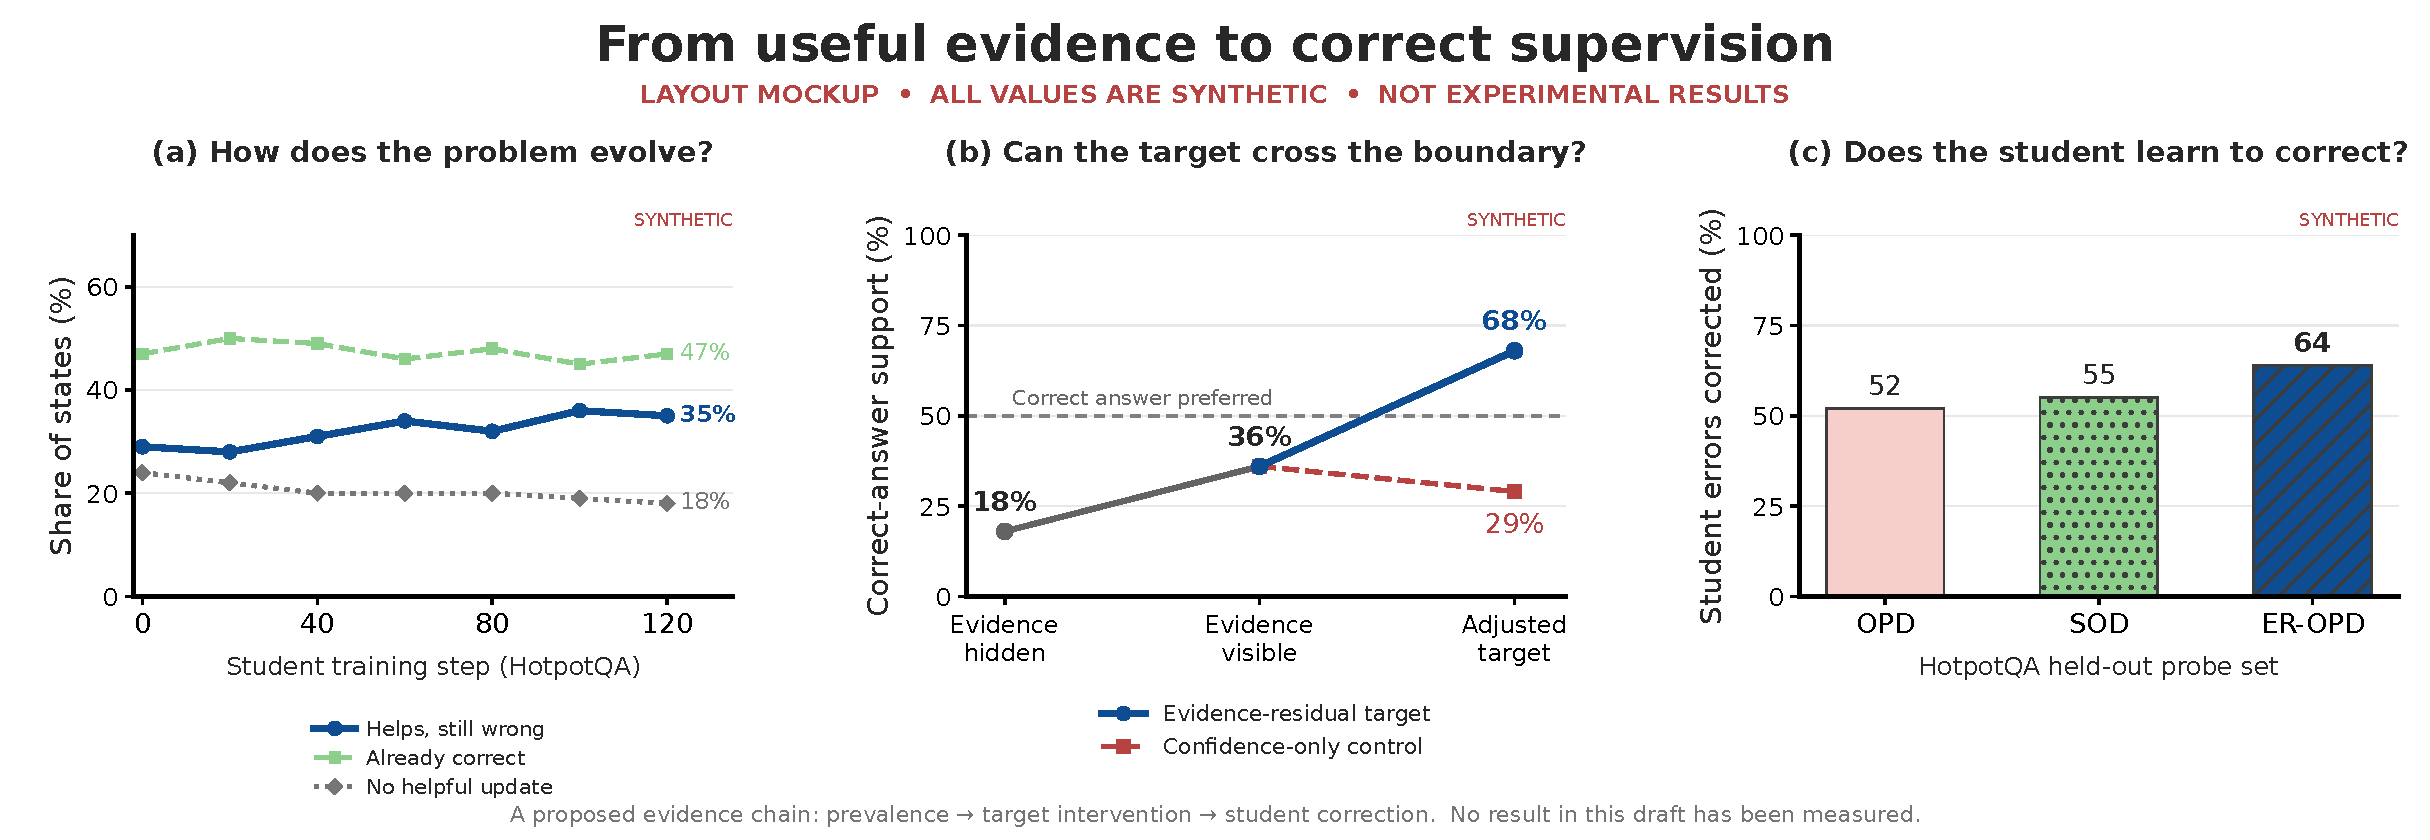
\includegraphics[width=\textwidth]{figures/er_story_mockup_20260915/er_story_SYNTHETIC_mockup.pdf}
\caption{\textbf{Synthetic layout mockup: all values are invented for design review.}
Proposed evidence chain for studying useful but insufficient evidence updates.
(a) Intended distribution across student training checkpoints of an OPD reference run trained only on HotpotQA, using the same diagnostic questions and frozen teacher. The x-axis denotes student optimizer updates, not teacher training or tool-interaction steps. The illustrative checkpoint positions are not a record of completed evaluations. The categories partition evidence-sufficient student states by the visible teacher's pairwise full-answer ranking and its change from the evidence-hidden view.
(b) Intended average correct-answer support within a fixed candidate set on states with helpful but insufficient updates. The 50\% line denotes equal support for the correct and competing wrong candidate sets, not a free-generation accuracy threshold. Lines connect evaluation conditions, not time steps. The control changes temperature to match target entropy without using answer labels.
(c) Intended correction rate on a HotpotQA held-out set of initially wrong student answers, selected using a common initial student and frozen teacher and held fixed across training methods.
No plotted prevalence, intervention effect, training outcome, or uncertainty estimate has been measured. This figure must not be used as empirical evidence.}
\end{figure*}
